\chapter{基于硅基反射微环的光调制器}
纯硅基光调制器的进展我们已经在第一章\ref{pure_simodulator}小结中有所总结。纯硅基光调制器目前都是采用调节波导折射率,从而改变谐振腔的谐振峰,或者改变马赫曾德两臂的相位差实现光强的调制。谐振腔型硅基光调制器,可以采用微环或者光子晶体结构。这类光调制器具有尺寸小,驱动电压低的特点,但是光学带宽受到谐振峰漂移量的限制。如果采用热调节微环谐振峰的位置,那么只有10~nm左右的漂移量。虽然微环光调制器可以通过增加尺寸,减小自由光谱范围(Free Spectra Range, FSR),实现宽光谱的调制,但是这样会增加微环光调制器的电容,减小调制带宽。增加尺寸也无助于降低驱动电压,这是由于微环光调制器谐振峰的偏移量$\Delta \lambda$由公式\ref{Equ:ring_tunning}决定。
\begin{equation}
\label{Equ:ring_tunning}
\frac{\Delta \lambda}{\lambda} = \frac{\Delta n_{eff}}{n_g}
\end{equation}
其中$\lambda$为工作波长,$\Delta n_{eff}$为等效折射率的改变量,$n_g$为波导的群速度。可以看出谐振峰的漂移量与微环的长度无关。因此,减小微环的驱动电压只能通过提高波导的电光响应,以及降低波导的群速度实现。

硅基等臂马赫曾德型光调制器具有光学带宽大,速度大的特点,但是尺寸大。由于硅基微弱的等离子色散效应,目前性能优异的马赫曾德光调制器至少需要2 mm的臂长作为调制区域,才能在0.36 V的差分驱动以下获得5 dB左右的消光比\cite{Ding2013electro}。对于等臂马赫曾德光调制器,输出光强$P_{out}$由公式\ref{Equ:mzi_tunning}决定。
\begin{equation}
\label{Equ:mzi_tunning}
P_{out} = \frac{1}{2}\left(1+cos\left(\frac{2\pi}{\lambda}\Delta n_{eff}L\right)\right)
\end{equation}
其中$L$为马赫曾德的臂长。相比与微环光调制器,降低马赫曾德光调制器的驱动电压,可以通过增加调制区域的长度来获得。不过,为了获得足够的消光比,驱动电压需要使马赫曾德光调制的调制区域有将近$\pi$的相位变化。

在本章中,我们提出在微环中集成马赫曾德型可调反射镜的结构,无需使调制区拥有$\pi$的相位变化就能实现高消光比的光调制器。这种新型光调制器的尺寸介于微环光调制器和马赫曾德型光调制器之间。它的FSR小,通过热调节也能实现宽光谱的调制。这种新型光调制器为实现低驱动电压,大光学带宽的纯硅基光调制器提供了新的设计思路。

在本章的内容组织上,首先我们对微环内反射的影响进行了理论分析。进而,我们在微环内加工光栅,研究不同反射率下,微环透射谱的变化。然后,我们分析可调反射镜的性质。最后,我们设计并且数值分析了在微环中集成可调反射镜的静态插入损耗,消光比和动态调制带宽。

\section{微环内反射的理论分析}
微环内反射对微环性能的影响可以从时域或者频域为切入点进行分析。以频域为切入点,需要采用传输矩阵模型\cite{yariv2006photonics}。而以时域为切入点,需要用时变的微分方程来分析\cite{haus1984waves}。由于频域模型下的传输矩阵模型需要考虑微环内部反射的具体结构,以及具体的工作波长,因此更适用于设计。而时域中的时变微分方程则更适合分析反射对微环的动态和静态性能的影响。下面我们首先介绍基于时变的微分方程法分析反射对微环透射谱的影响\cite{haus1984waves,Li2016design,little1997microring}。
\begin{figure}[htb]
	\centering
	\includegraphics[width=6cm]{./Pictures/chapt5_ring_reflector_structure.jpg}
	\caption{在时域耦合模式理论(tCMT)下,有内部反射的微环模型。其中正向传播的光振幅$\alpha_+$和反向传播的光振幅$\alpha_-$,在反射处相互耦合}
	\label{chapt5_ring_reflector_structure}
\end{figure}

基于时变的微分方程法又称作时域耦合模式理论(Temporal Coupled Mode Theory, tCMT)。当微环内部有反射时,微环内部就会有两个方向传播的光模式,如图\ref{chapt5_ring_reflector_structure}所示。我们根据其传播的方向,将其正向传播的幅值记为$\alpha_+$,将反向传播的幅值记为$\alpha_-$。而$|\alpha_+|^2$和$|\alpha_-|^2$表示正向传播和反向传播模式的能量。当微环中有反射时,这两个模式在反射处相互耦合,从而影响了微环的正常输出光谱,使其消光比发生变化,甚至谐振模式产生了劈裂。如果用tCMT方程描述这种情况就如公式\ref{Equ:alpha_ccw},公式\ref{Equ:alpha_cw}和公式\ref{Equ:St_Sr}所示\cite{Li2016design}。
\begin{equation}
\label{Equ:alpha_ccw}
\frac{d\alpha_+}{dt}=j\omega_r\alpha_+-\left(\frac{1}{\tau_i}+\frac{1}{\tau_l}\right)\alpha_+-j\mu_iS_i-j\mu_r\alpha_-
\end{equation}
\begin{equation}
\label{Equ:alpha_cw}
\frac{d\alpha_-}{dt}=j\omega_r\alpha_--\left(\frac{1}{\tau_i}+\frac{1}{\tau_l}\right)\alpha_--j\mu_r^*\alpha_+
\end{equation}
\begin{equation}
\label{Equ:St_Sr}
S_t = S_i-j\mu_i\alpha_+ ~~~~~~~~~~~~ S_r = -j\mu_i\alpha_-
\end{equation}
其中$\omega_r$是微环的谐振频率。$S_i$表示输入光的振幅。$1/\tau_i$表示微环中光场耦合到波导导致的能量衰减率。$1/\tau_l$表示微环中的光场由于微环本身弯曲和材料等损耗$\alpha_l$导致的能量衰减率。$\mu_i$是波导和微环的波导耦合强度。$\mu_r$是$\alpha_+$和$\alpha_-$的反射耦合强度。其中,波导耦合强度$\mu_i$与衰减率$\tau_i$,损耗系数$\alpha_l$与衰减率$\tau_l$,反射耦合强度$\mu_r$与光场反射率$r$的关系分别如公式\ref{Equ:mu_tau}所示\cite{little1997microring}。
\begin{equation}
\label{Equ:mu_tau}
\mu_i^2=k_i^2\frac{c}{n_gL}=\frac{2}{\tau_i}~~~~~~~~~~~~\alpha_l^2\frac{c}{n_gL}=\frac{2}{\tau_l}~~~~~~~~~~~~\mu_r^2=r^2\frac{c}{n_gL}^2
\end{equation}
其中$c$是真空中的光速,$n_g$是波导的群折射率,$L$是微环的周长。通过解公式\ref{Equ:alpha_ccw}、公式\ref{Equ:alpha_cw}和公式\ref{Equ:St_Sr},对于角频率为$\omega_0$的输入光场$S_i$,我们可以获得波导输出光场$S_t$,见公式\ref{Equ:St}所示。
\begin{equation}
\label{Equ:St}
\frac{S_t}{S_i}=1-\frac{1}{\tau_i}\left(\frac{1}{j(\omega_0-\omega_1)+(1/\tau_i+1/\tau_l)} + \frac{1}{j(\omega_0-\omega_2)+(1/\tau_i+1/\tau_l)}\right)
\end{equation}

可以看到,此时输出光谱需要用两个洛仑兹线形(Lorentzian-shape)进行拟合,而传统的微环,只需要一个洛仑兹线性。两个洛仑兹线形的中心频率分别为$\omega_1 = \omega_r+|\mu_r|$,$\omega_2=\omega_r-|\mu_r|$。中心频率的偏移量正比于微环的反射耦合强度$\mu_r$,也就是中间反射器的反射强度$r$。在两个谐振频率出的透射率$P_r$如公式\ref{Equ:Pr}所示。
\begin{equation}
\label{Equ:Pr}
P_r = \left|\frac{S_t}{S_i}\right|^2_{\omega = \omega_1~or~\omega_2}= \left(\frac{\alpha_l^2}{k_i^2+\alpha_l^2}\right)^2+\frac{(k_i^4-2k_i^2\alpha_l^2)}{(k_i^2+\alpha_l^2)^2+16r^2}
\end{equation}
当$r=0$时,公式\ref{Equ:Pr}就变成了普通微环的谐振频率处的透射率:
\begin{equation}
\label{Equ:Pr_no_r}
P_r=\left(\frac{\alpha_l^2-k_i^2}{k_i^2+\alpha_l^2}\right)^2
\end{equation}
当$k_i = \alpha_l$时,微环处于临界工作点,$k_i$称为临界耦合系数$k$。此时,普通微环在谐振频率处的透射率达到最小值0。而当微环内有反射时,谐振峰处的透射谱将与反射率$r$有关,如公式\ref{Equ:Pr_critical_r}所示。微环在谐振峰处的消光比我们采用公式\ref{Equ:RingER}的定义。
\begin{equation}
\label{Equ:RingER}
ER_{ring}=-10 \times log_{10}(Pr)
\end{equation}
\begin{equation}
\label{Equ:Pr_critical_r}
P_r=\frac{1}{4}-\frac{k_i^4}{4k_i^2+16r^2}
\end{equation}
\begin{figure}[htb]
	\centering
	\includegraphics[width=12cm]{./Pictures/chapt5_r_k_Ex_alpha1e-2.eps}
	\caption{当微环损耗$\alpha_l^2= 10^{-2}$时,谐振峰处的消光比与耦合系数$k_i^2$,内部反射率$r^2$的关系}
	\label{chapt5_r_k_Ex_alpha1e-2}
\end{figure}
\begin{figure}[htb]
	\centering
	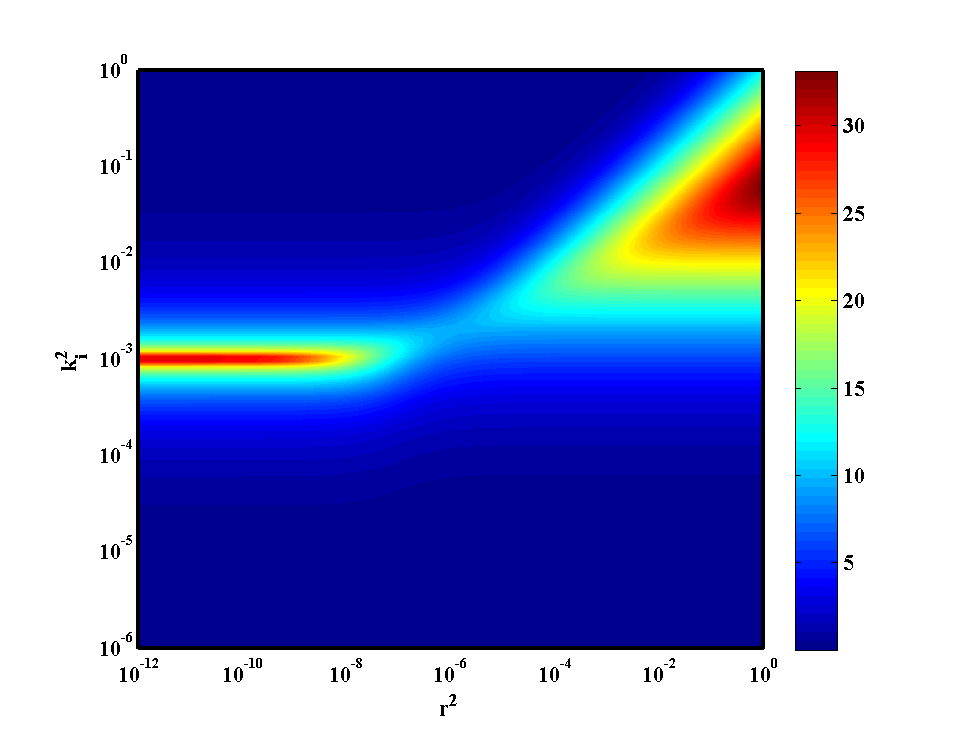
\includegraphics[width=12cm]{./Pictures/chapt5_r_k_Ex_alpha1e-3.eps}
	\caption{当微环损耗$\alpha_l^2= 10^{-3}$时,谐振峰处的消光比与耦合系数$k_i^2$,内部反射率$r^2$的关系}
	\label{chapt5_r_k_Ex_alpha1e-3}
\end{figure}
\begin{figure}[htb]
	\centering
	\includegraphics[width=12cm]{./Pictures/chapt5_r_k_Ex_alpha1e-4.eps}
	\caption{当微环损耗$\alpha_l^2= 10^{-4}$时,谐振峰处的消光比与耦合系数$k_i^2$,内部反射率$r^2$的关系}
	\label{chapt5_r_k_Ex_alpha1e-4}
\end{figure}
图\ref{chapt5_r_k_Ex_alpha1e-2},\ref{chapt5_r_k_Ex_alpha1e-3},\ref{chapt5_r_k_Ex_alpha1e-4}展示了,在不同损耗$\alpha_l$的微环中,$k_i$,$r$对谐振频率处的消光比的影响。从图\ref{chapt5_r_k_Ex_alpha1e-2}可以看到,当微环的损耗很大($\alpha_l^2 = 10^{-2}$)时,微环内部存在微弱的反射时($r^2<10^{-7}$),对$k_i$与消光比的关系影响很弱,依旧是在$k_i=\alpha_l$时存在最大的消光比。不过此时,临界耦合处的消光比,随着反射率的增大而减弱。当微环内部存在的反射率继续增大时,$k_i$的变化对消光比的影响逐渐弱。而且谐振峰消光比最大处满足的条件不再是$k_i = \alpha_l$,而是$k_i > \alpha_l$,并且随着$r$的增加对应的$k_i$继续增大。

当微环内部损耗降低到$\alpha_l^2 = 10^{-3}$时,从图\ref{chapt5_r_k_Ex_alpha1e-3}可以看到,微环对内部的反射敏感。只有当$r^2<10^{-8}$时,微环才能保持原先的$k_i$与消光比的关系。当微环内部的反射率继续增加到$r>10^{-4}$时,谐振峰的消光比最大时的$k_i$也是随着$r$的增加而增大。并且相比于$r^2<10^{-8}$时,高的消光比只存在很窄的$k_i\approx k_i$区域,而当$r^2>10^{-2}$,高的消光比对应更宽的$k_i$区域。

当微环的内部损耗继续降低到$\alpha_l^2=10^{-4}$时,从图\ref{chapt5_r_k_Ex_alpha1e-4}可以看到,微环对内部反射更加敏感。在临界耦合处的微环只需要引入极小的反射{$r^2\approx 10^{-10}$},消光比就会有很大的改变。而当$r>10^{-6}$时,谐振峰的消光比最大时对应的$k_i$和$r$的变化几乎成线性关系。$r^2>10^{-2}$时,高的消光比存在的区域比之前高损耗的情况下,面积更大。

微环内反射引起反射谱变化的现象,已经被研究人员所利用。在超低损耗微盘中,利用微小颗粒附着微盘引起微盘内部微小的反射,从而使实现对半径只有30~nm纳米颗粒的检测\cite{zhu2010chip}。而对于当微环内部反射率很大时,高消光比的微环对耦合系数不敏感的现象,我们可以用于实现工艺容差大的光波长滤波器\cite{qiangsheng2015fsr}。

我们在本论文中,我们将通过调制微环内部反射率从而实现光调制器。不过下面我们先将对这个理论现象进行实验的验证。
\section{含内部反射的微环的设计与实验}
\begin{figure}[htb]
	\centering
	\includegraphics[width=12cm]{./Pictures/chapt5_ring_grating_reflector_structure.jpg}
	\caption{利用光栅结构在微环内引入反射的结构示意图}
	\label{chapt5_ring_grating_reflector_structure}
\end{figure}

在实验分析微环内反射的影响时,我们也分析了不同反射强度和耦合系数对微环透射谱的影响。我们通过将微环内部加入光栅,具体结构示意图如图\ref{chapt5_ring_grating_reflector_structure}所示,从而引入反射。通过改变反射光栅的尺寸,调节反射强度。而波导与微环的耦合系数则通过波导和微环的距离调节。
\subsection{结构参数设计和仿真}
在设计这个结构时,我们采用的是频域的传输矩阵法\cite{yariv2006photonics}。在图\ref{chapt5_ring_grating_reflector_structure}中的全局图中,$\tau$是波导的自耦合系数,$\kappa$是交叉耦合系数,$R$是微环半径。$\tau$和$\kappa$满足能量守恒关系$\tau^2+\kappa^2=1$。在光栅的第$i$个周期的局部小图中,$A_i, B_i$分别是正向和反向传播模式的振幅。$\Lambda$是光栅的周期,$l_g$是光栅齿的宽度,$h_g$是光栅齿的高度,$r$是单个光栅界面的反射率。另外我们定义光栅的占空比$D=l_g/\Lambda$。

当$N$个光栅均匀分布在整个微环时,对于微环中m阶的谐振波长$\lambda_m$,若$N = 2m$,则谐振波长$\lambda_m$正好是光栅反射谱的中心波长。这是由于第m阶的谐振波长满足公式\ref{Equ:lambdam}:
\begin{equation}
\label{Equ:lambdam}
m\lambda_m = 2n_{n_{eff}}\pi R
\end{equation}
其中$n_{eff}$为波导在$\lambda_m$的等效折射率。若$N=2m$,则公式\ref{Equ:lambdam}可以写成:
\begin{equation}
\label{Equ:grating}
\frac{\lambda_m}{2}=\frac{2n_{eff}\pi R}{N}=n_{eff}\Lambda.
\end{equation}

公式\ref{Equ:grating}说明$\lambda_m$此时正好是光栅的布拉格波长(Bragg wavelength),处于反射谱的中心。我们通过调节光栅的尺寸,进而调节$\lambda_m$处反射率的大小。而微环其他的谐振波长则不受到光栅反射的影响。 

接下来,我们详细介绍利用传输矩阵计算包含光栅的微环的透射谱的方法。微环的传输矩阵可以写成公式\ref{Equ:ring_TMM}所示:
\begin{equation}
\label{Equ:ring_TMM}
\begin{bmatrix}
S_{i}\\
S_{t}
\end{bmatrix} =\frac{1}{k}\begin{bmatrix}
1 & -\tau\\
\tau & -1
\end{bmatrix}
\begin{bmatrix}
A_{1}\\
A_{n+1}
\end{bmatrix}
\end{equation}

我们假设$A_1$与$A_{n+1}$的关系为$A_1=f(A_{n+1})$,那么微环的透射谱为公式\ref{Equ:ring_TMM_T}。
\begin{equation}
\label{Equ:ring_TMM_T}
\frac{S_t}{S_i}=\frac{\tau f(A_{n+1})-A_{n+1}}{f(A_{n+1})-\tau A_{n+1}}
\end{equation}

我们再根据光栅的传输矩阵方程,计算得到$f(A_{n+1})$的形式。在第i个光栅周期中$A_i$,$B_i$,$A_{i+1}$,$B{i+1}$的关系如下:
\begin{equation}
\label{Equ:ithTMM}
\begin{bmatrix}
A_{i}\\
B_{i}
\end{bmatrix} 
=
\frac{1}{1-r^2}
\begin{bmatrix}
1 & r\\
r & 1
\end{bmatrix}
\begin{bmatrix}
e^{i\phi_1} & 0 \\
0 & e^{-i\phi_1}
\end{bmatrix}
\begin{bmatrix}
1 & r\\
r & 1
\end{bmatrix}
\begin{bmatrix}
e^{i\phi_2} & 0 \\
0 & e^{-i\phi_2}
\end{bmatrix}
\begin{bmatrix}
A_{i+1}\\
B_{i+1}
\end{bmatrix} 
\end{equation}
其中$\phi_1=D\pi/2$,$\phi_2=(1-D)\pi/2$。我们将中间的四个矩阵形式相乘,可以简化为公式\ref{Equ:ring_TMM_sim}的形式。
\begin{equation}
\label{Equ:ring_TMM_sim}
\begin{bmatrix}
A_{i}\\
B_{i}
\end{bmatrix} 
=
\begin{bmatrix}
m_{11} & m_{12}\\
m_{21} & m_{22}
\end{bmatrix}
\begin{bmatrix}
A_{i+1}\\
B_{i+1}
\end{bmatrix}
\end{equation}

我们只需要把N个周期的光栅矩阵相乘就可以获得如$A_1$,$B_1$,$A_{N+1}$,$B_{N+1}$的关系:
\begin{equation}
\label{Equ:ring_TMM_multi}
\begin{bmatrix}
A_{1}\\
B_{1}
\end{bmatrix} 
=
\begin{bmatrix}
m_{11} & m_{12}\\
m_{21} & m_{22}
\end{bmatrix}^N
\begin{bmatrix}
A_{N+1}\\
B_{N+1}
\end{bmatrix}
=
\begin{bmatrix}
M_{11} & M_{12}\\
M_{21} & M_{22}
\end{bmatrix}
\begin{bmatrix}
A_{N+1}\\
B_{N+1}
\end{bmatrix}
=
\textbf{M}
\begin{bmatrix}
A_{N+1}\\
B_{N+1}
\end{bmatrix}
\end{equation}

利用布洛赫波(Bloch Wave)的方法\cite{yariv2006photonics},我们将最后的\textbf{M}矩阵写为:
\begin{equation}
\label{Equ:ring_bloch}
\textbf{M}
=
\begin{bmatrix}
m_{11}U_{N-1} - U_{N-1}& m_{12}U_{N-1}\\
m_{21}U_{N-1} & m_{22}U_{N-1}-U_{N-2}
\end{bmatrix}
\end{equation}
其中,
\begin{equation}
\label{Equ:UN}
U_N = \frac{sin((N+1)K\Lambda)}{sin(K\Lambda)}
\end{equation}
\begin{equation}
\label{Equ:KLambda}
K\Lambda = cos^{-1}\left(\frac{m_{11}+m_{22}}{2}\right)
\end{equation}

为了求解$A_1$与$A_{N+1}$的关系,我们还需要$B_{1}$与$B_{N+1}$的关系,如公式\ref{Equ:B1BN1}所示。
\begin{equation}
\label{Equ:B1BN1}
B_{N+1} = \tau B_1 
\end{equation}
利用公式\ref{Equ:ring_TMM_multi},\ref{Equ:ring_bloch},\ref{Equ:UN},\ref{Equ:KLambda},\ref{Equ:B1BN1}我们可以获得$A_1$与$A_{N+1}$的关系如公式\ref{Equ:A1relationAN}所示。
\begin{equation}
\label{Equ:A1relationAN}
A_1 = \frac{M_{11}-\tau |\textbf{M}|}{1-\tau M_{22}}A_{N+1}
\end{equation}
将公式\ref{Equ:A1relationAN}代入公式\ref{Equ:ring_TMM_T}我们就可以得到公式\ref{Equ:ring_grating_T},用于计算含光栅微环的透射谱。
\begin{equation}
\label{Equ:ring_grating_T}
\frac{S_t}{S_i}=\frac{\tau M_{11} + \tau M_{22} - \tau^2|\textbf{M}|-1}{M_{11}+\tau^2 M_{22}-2\tau}
\end{equation}
\begin{figure}[htb]
	\small
	\subfigure[]{
		\begin{minipage}[]{0.5\textwidth}
			\centering
			\label{chapt5_grating_ring_single_small}
			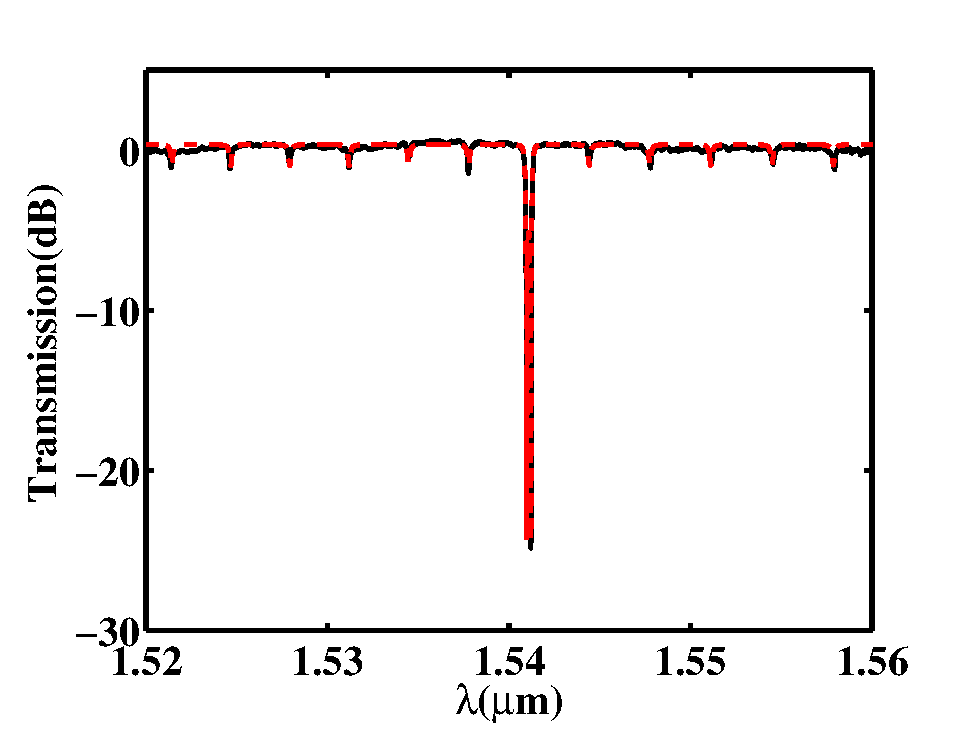
\includegraphics[width=8cm]{./Pictures/chapt5_grating_ring_single.eps}
		\end{minipage}}
	\subfigure[]{
		\begin{minipage}[]{0.5\textwidth}
			\centering
			\label{chapt5_grating_ring_single_large} %% label for second subfigure
			\includegraphics[width=8cm]{./Pictures/chapt5_grating_ring_single_large.eps}
		\end{minipage}}
	\caption{含光栅的微环的实验和理论的透射谱,其中红色虚线是理论计算结果,黑色实线是实验测试结果:(a)包含不同微环谐振波长的透射谱;(b)与光栅布拉格波长相同的谐振波长的局部放大图}
	\label{chapt5_grating_ring_single}	
\end{figure}

图\ref{chapt5_grating_ring_single}展示了,半径30~$\mu m$的光栅微环透射谱。其中红虚线部分是按公式\ref{Equ:ring_grating_T}计算的结果。而黑实线则是实验测试的结果。光栅的个数$N = 658$,对应的谐振波长$\lambda = 1541.1~nm$,占空比$D = 0.2$, 品质因子$Q = 100,000$,自耦合系数$\tau = 0.87$,单个周期的反射率$r = 0.000335$。从图\ref{chapt5_grating_ring_single_small}中可以看出,由于光栅只在谐振波长1541.1~nm处有反射,因此,此处谐振波长的消光比与没有反射影响的谐振峰的消光比有很大不同。由于微环Q值比较高,而此时自耦合系数比较小(意味着交叉耦合系数$k$远大于临界耦合系数),根据图\ref{chapt5_r_k_Ex_alpha1e-4}可以知道,因此在1541.1~nm处大的反射率能引起此时较大的消光比。从图\ref{chapt5_grating_ring_single_large}可以看到理论计算结果和实际测试结果十分吻合。

\subsection{结构制作和实验结果}
\begin{figure}[htb]
	\centering
	\includegraphics[width=12cm]{./Pictures/chapt5_ring_grating_reflector_structure_real.jpg}
	\caption{含光栅的微环的电镜图,右图是局部放大图}
	\label{chapt5_ring_grating_reflector_structure_real}
\end{figure}
包含光栅的微环结构,我们是采用电子束光刻机定义图形。工艺流程与第五章\ref{fab_siwg}小结相同。SOI最上层硅的厚度是220~nm。为了防止光栅结构引起微环侧壁粗糙导致损耗,我们采用浅刻蚀70~nm宽度为600~nm的脊形波导。光栅和微环是同时用电子束光刻机定义的,无需套刻。最后加工完成的器件电镜图如图\ref{chapt5_ring_grating_reflector_structure_real}所示。我们也在输入输出波导端加上光栅耦合结构,用于和光纤的耦合。

\begin{figure}[htb]
	\centering
	\includegraphics[width=12cm]{./Pictures/chapt5_ring_grating_vary_reflector.jpg}
	\caption{(a)含光栅的微环的透射谱随不同反射率的关系,其中黑实线是实验测试的结果,红虚线是理论计算的结果;(b)和(c)分别是理论计算得的两个峰之间劈裂的距离和消光比随反射率的关系}
	\label{chapt5_ring_grating_vary_reflector}
\end{figure}

图\ref{chapt5_ring_grating_vary_reflector}(a)展示的透射谱的变化是通过控制光栅的尺寸参数$h_g$从30~nm变化到80~nm来实现的,对应的单个周期的反射率是从0.0001736变化到0.00132。由于光栅尺寸的变化,以及工艺的不稳定性,谐振峰的波长会有所漂移。从图\ref{chapt5_ring_grating_vary_reflector}(b)我们可以看到当反射率增大时,谐振峰劈裂的间隔也会增加。虽然,在反射率小于一个临界值$r_c$的时候,谐振峰看起来只有一个,没有劈裂,其实这是两个洛仑兹线性的谐振峰叠加在一起形成的。图\ref{chapt5_ring_grating_vary_reflector}(c)展示的反射率与消光比的关系,从中我们可以到,刚开始消光比对反射十分敏感。当反射率达到临界的$r_c$时,透射谱的消光比达到最高,并且随着反射率的增加,反射率将稳定在一个值。这个现象与我们之前用时域微分法的图\ref{chapt5_r_k_Ex_alpha1e-4}的有所差别。这是由于这里的反射率是单个周期的反射率,而图\ref{chapt5_r_k_Ex_alpha1e-4}的反射率是个整体的反射率。并且用频域的传输矩阵法,整体光栅的反射率将不仅包含对光振幅的反射,还有对光相位的影响,而图\ref{chapt5_r_k_Ex_alpha1e-4}的反射率仅包含对光幅度的影响。因此,对于含光栅的微环结构,图\ref{chapt5_ring_grating_vary_reflector}(c)比图\ref{chapt5_r_k_Ex_alpha1e-4}的精确度更高。

\begin{figure}[htb]
	\centering
	\includegraphics[width=12cm]{./Pictures/chapt5_ring_grating_vary_tau.jpg}
	\caption{(a)含光栅的微环的透射谱随不同自耦合系数$\tau$的关系,其中黑实线是实验测试的结果,红虚线是理论计算的结果;(b)和(c)分别是理论计算得的两个峰的劈裂距离和消光比随自耦合系数$\tau$的关系}
	\label{chapt5_ring_grating_vary_tau}
\end{figure}

接下来,我们还分析了含光栅的微环的自耦合系数$\tau$的变化对透射谱的影响。我们将波导和微环的间隔从50~nm变化到300~nm,使其对应的自耦合系数$\tau$从0.3变化到0.9,即交叉耦合系数$\kappa$则从0.954变化到0.435。图\ref{chapt5_ring_grating_vary_tau}(a)展示了透射谱随着自耦合系数变化的关系。图\ref{chapt5_ring_grating_vary_tau}(b)中展示了,随着自耦合系数$\tau$的增加,刚开始两个劈裂的波长距离近,无法分辨。但是超过一个临界值$\tau_c$后,两个劈裂波长之间的距离,随着自耦合系数的增大而逐渐增加。当$\tau$趋向于1时,劈裂波长之间的距离将趋向于饱和。从图\ref{chapt5_ring_grating_vary_tau}(c),我们可以看到随着自耦合系数$\tau$的增加,劈裂波长处的消光比先逐渐增加。当自耦合系数达到相同临界点$\tau_c$时,含光栅的微环的消光比达到最高。当自耦合系数超过$\tau_c$时,消光比又会回落。在图\ref{chapt5_ring_grating_vary_tau}(c)中的红线是不含反射的普通微环的消光比随自耦合系数的关系。通过比较,我们可以得到,微环中引入反射,将会使更大范围的自耦合系数$\tau$拥有高的消光比。

通过比较图\ref{chapt5_ring_grating_vary_reflector}(b)和图\ref{chapt5_ring_grating_vary_tau}(b)我们可以发现,反射率$r$的大小决定了当自耦合系数趋向于1时,谐振峰劈裂的最大距离。通过比较图\ref{chapt5_ring_grating_vary_reflector}(c)和图\ref{chapt5_ring_grating_vary_tau}(c)我们可以发现自耦合系数$\tau$决定了当反射率大于临界值$r_c$时,最后的饱和消光比。

如果利用微环加光栅的结构制作调制器,我们可以通过调节每个周期的反射率$r$,根据图\ref{chapt5_ring_grating_vary_reflector}(c),使其工作在临界点$r_c$附近。但是制作这种结构的硅基光调制器,不仅对电极套刻要求很高,而且由于光栅宽度只有30~nm到80~nm,对掺杂的精度要求也高。这驱使我们设计新的结构以实现微环内部的反射率可调。

\section{基于硅基可调反射镜的设计} \label{tunable_reflector}
\begin{figure}[htb]
	\centering
	\includegraphics[width=12cm]{./Pictures/chapt5_tunable_reflection_mirror.jpg}
	\caption{硅基可调反射镜的结构示意图}
	\label{chapt5_tunable_reflection_mirror}
\end{figure}
\begin{figure}[htb]
	\centering
	\includegraphics[width=15cm]{./Pictures/chapt5_tunable_reflection_mirror_inter.jpg}
	\caption{硅基可调反射镜在Intercoonnect\cite{interconnect}中的拆解示意图}
	\label{chapt5_tunable_reflection_mirror_inter}
\end{figure}
我们利用输出端为回路反射镜(Loop Mirror)的马赫曾德干涉器作为可调反射镜\cite{Li2016design},结构示意图见图\ref{chapt5_tunable_reflection_mirror}所示,其中两臂的相位分别是$\phi_1$和$\phi_2$。我们采用的马赫曾德干涉器两臂光学长度初始状态下相等$\phi_1 = \phi_2$,通过调制其中一臂的相位,就可以实现反射谱的强度变化。我们采用商业软件Lumerical中基于散射矩阵计算多个级联光学器件性能的Interconnect\cite{interconnect}模块对可调反射镜的性能进行计算。可调反射镜可以分解成三个基本光学器件:3~dB耦合器,直波导和马赫曾德两臂上的相位调制波导,具体在Interconnect中的分解如图\ref{chapt5_tunable_reflection_mirror_inter}所示。
\begin{figure}[htb]
	\centering
	\includegraphics[width=16cm]{./Pictures/chapt5_tunable_reflection_mirror_spec.jpg}
	\caption{硅基可调反射镜的反射(R)谱和透射(T)谱:(a)当两臂的光程差相等;(b)当两臂的光程差相差$\pi$}
	\label{chapt5_tunable_reflection_mirror_spec}
\end{figure}
\begin{figure}[htb]
	\centering
	\includegraphics[width=10cm]{./Pictures/chapt5_tunable_reflection_mirror_spec_single.jpg}
	\caption{硅基可调反射镜在1540~nm处的反射率随其中一臂折射率变化的关系}
	\label{chapt5_tunable_reflection_mirror_spec_single}
\end{figure}

我们采用的直波导,以及两臂上的相位调制波导的尺寸,都是依据Imec代工厂提供的数据\cite{Imec}。硅的直波导的参数是,220~nm厚深刻蚀450~nm宽的条形波导,其在1540~nm处的等效折射率$n_{eff}$为2.368,群折射率$n_{g}$为4.329,损耗是0.2~dB/mm。相位调制波导的参数是,215~nm厚浅刻蚀155~nm,450~nm宽的脊形波导。其在1540~nm处的等效折射率$n_{eff}$为2.450,群折射率$n_{g}$为4.0367,损耗是2.5~dB/mm。我们假设马赫曾德两臂上的相位调制波导的长度都为200~$\mu m$,回路反射镜的长度为50 $\mu m$,并且3~dB耦合器是理想的能量均分的耦合器,那么当在两臂不同的光程差分别为0和$\pi$时,可调反射镜反射谱和透射谱如图\ref{chapt5_tunable_reflection_mirror_spec}所示。可以看到,改变两臂的相位差,仿真的反射谱和透射谱既宽又平坦。器件的最大反射率受到波导损耗影响只有0.8。接下来,我们扫描其中一个相位调制波导的等效折率,分析两臂的等效折射率差$\Delta n_{eff}$与1540~nm处的反射率和透射率的关系,如图\ref{chapt5_tunable_reflection_mirror_spec_single}所示。可以看到,当$\Delta n_{eff}$变化时,反射率和透射率的变化趋势是正弦函数,$\Delta n_{eff}$的变化周期为0.00385。

\begin{figure}[htb]
	\centering
	\includegraphics[width=15cm]{./Pictures/chapt5_tunable_reflection_mirror_flatten.jpg}
	\caption{硅基可调反射镜展开成两个级联的马赫曾德的结构图。中间波导的长度为回路反射镜的长度,右边马赫曾德的两臂长度与左面马赫曾德的两臂长度互换}
	\label{chapt5_tunable_reflection_mirror_flatten}
\end{figure}
虽然商业软件能给我们准确的计算结果,但是我们无法直观了解,通过调整哪些参数能够改变器件的性能。在此,我们采用频域的传输矩阵计算可调反射镜的频谱响应,分析具体哪些参数能影响反射率。首先我们对可调反射镜的结构,如图\ref{chapt5_tunable_reflection_mirror}所示,进行镜像展开,等效成两个级联的马赫曾德结构,如图\ref{chapt5_tunable_reflection_mirror_flatten}所示。左边马赫曾德的上下两臂引入的相位分别是$\phi_1$,$\phi_2$。而由于回路反射镜的关系,右边马赫曾德的上下两臂引入的相位分别是是$\phi_2$, $\phi_1$。在理想的3~dB耦合器,无损耗的波导情况下,两个级联马赫曾德的传输矩阵如公式\ref{Equ:three_MZI}所示。
\begin{equation}
\label{Equ:three_MZI}
\begin{bmatrix}
t\\
r
\end{bmatrix}
= e^{i(\phi_1+\phi_2)}
\begin{bmatrix}
-cos(\Delta \phi) & sin(\Delta \phi)\\
-sin(\Delta \phi) & -cos(\Delta \phi)
\end{bmatrix}
\begin{bmatrix}
E_{in}\\
0
\end{bmatrix}
\end{equation}
其中,$\Delta \phi = \phi_1-\phi_2$,$E_{in}$为输入光的振幅。根据公式\ref{Equ:three_MZI},我们可以获得透射$T$和反射$R$的表达式分别为:
\begin{equation}
\label{Equ:tunable_T}
T = |t|^2 = cos(\Delta \phi)^2 |E_{in}|^2 = \frac{1+cos(\Delta n_{eff}\frac{4\pi L}{\lambda})}{2}|E_{in}|^2
\end{equation}
\begin{equation}
\label{Equ:tunable_R}
R = |r|^2 = sin(\Delta \phi)^2 |E_{in}|^2= \frac{1-cos(\Delta n_{eff}\frac{4\pi L}{\lambda})}{2}|E_{in}|^2
\end{equation}
其中,$\Delta n_{eff}$为两臂的等效折射率差,$L$为臂长,$\lambda$是工作波长。从公式\ref{Equ:tunable_T}和公式\ref{Equ:tunable_R}可以看出,$T$和$R$随等效折率差的变化趋势与我们用Interconnect软件仿真所得的图\ref{chapt5_tunable_reflection_mirror_spec_single}相同。反射率随等效折射率差的变化周期为$\lambda/2L$。当$\lambda = 1540~nm, L = 200~\mu m$时,周期为0.00385,与图\ref{chapt5_tunable_reflection_mirror_spec_single}中所示的相同。

\begin{figure}[htb]
	\centering
	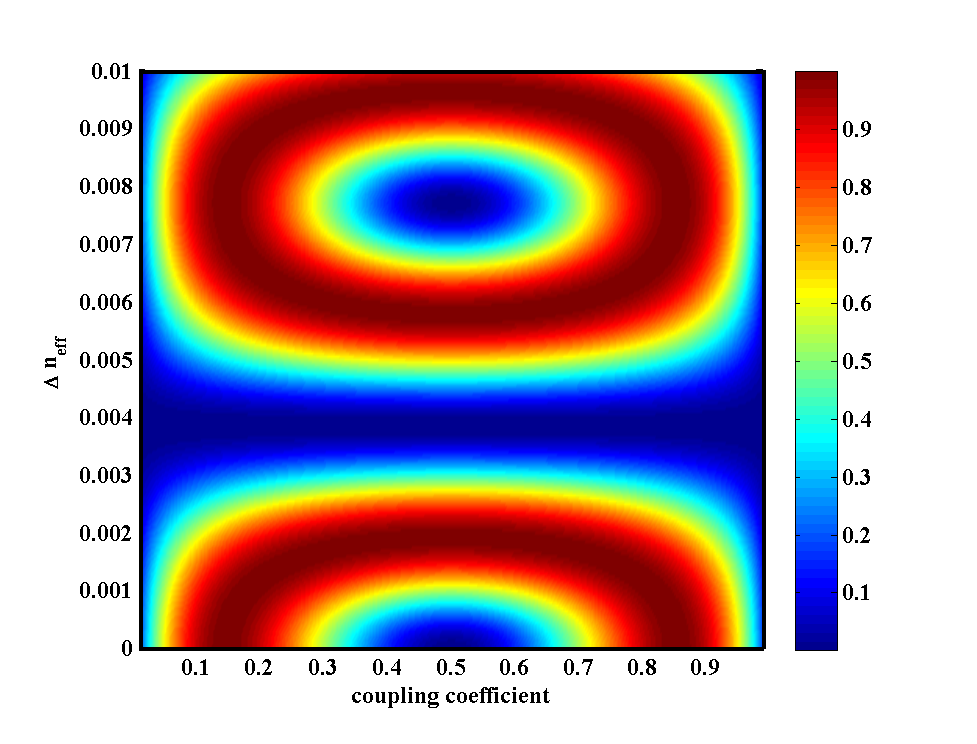
\includegraphics[width=15cm]{./Pictures/chapt5_grating_ring_real_3dB.eps}
	\caption{对于可调反射镜,当耦合器的耦合率(coupling coefficient)变化时,改变两臂的等效折射率差$\Delta n_{eff}$对可调反射镜反射率的影响。}
	\label{chapt5_grating_ring_real_3dB}
\end{figure}
我们进一步分析了,当实际加工的3~dB耦合器并非理想的将能量均分时,对可调反射器性能的影响。由于在实验中,两个耦合器的结构相同,工艺步骤相同,因此我们默认两者的耦合效率(coupling coefficient)始终保持一样。 图\ref{chapt5_grating_ring_real_3dB}可以看出,当耦合效率在0.85至0.15之间变化时,通过调节两臂的等效折射率差,依旧能使可调反射镜达到全反射和全透过的工作点。这表明了这个可调反射镜具有很大的工艺容差。下面我将使用这个可调反射镜与微环相结合实现新型的硅基可调反射镜的微环光调制器。

\section{基于硅基可调反射镜的微环光调制器的设计}
\begin{figure}[htb]
	\centering
	\includegraphics[width=12cm]{./Pictures/chapt5_tunable_reflection_ring_structure.jpg}
	\caption{硅基可调反射镜的微环光调制器的结构示意图}
	\label{chapt5_tunable_reflection_ring_structure}
\end{figure}
我们将可调反射镜与微环相结合的结构如图\ref{chapt5_tunable_reflection_ring_structure}所示。当默认状态下可调反射镜的反射率为0,微环在谐振波长处有最大的消光比,当我们调制可调反射镜的一臂的等效折射率,使可调反射镜的反射率非0时,从而使改变微环的输出谱,实现光强的调制。从图\ref{chapt5_r_k_Ex_alpha1e-2},图\ref{chapt5_r_k_Ex_alpha1e-3},图\ref{chapt5_r_k_Ex_alpha1e-4}可以看出,当微环的损耗越小,Q值越高时,内部反射导致的微环透射谱的变化越明显。

我们设计的硅基可调反射镜中的相位调制区域有200~$\mu m$,介于微环调制和马赫曾德调制器的中间。这种新型光调制器相比硅基马赫曾德光调制,无需实现相位调制区$\pi$相位的变化,就能实现高消光比。相比于微环光调制器,可以通过增加调制区域的长度,减小驱动电压。另外,借助于可调反射镜宽光谱反射的特点,通过热调微环谐振峰,使这种新型光调制器有大的光学工作带宽。下面我们将详细介绍设计过程和调制带宽的仿真。

\begin{figure}[htb]
	\centering
	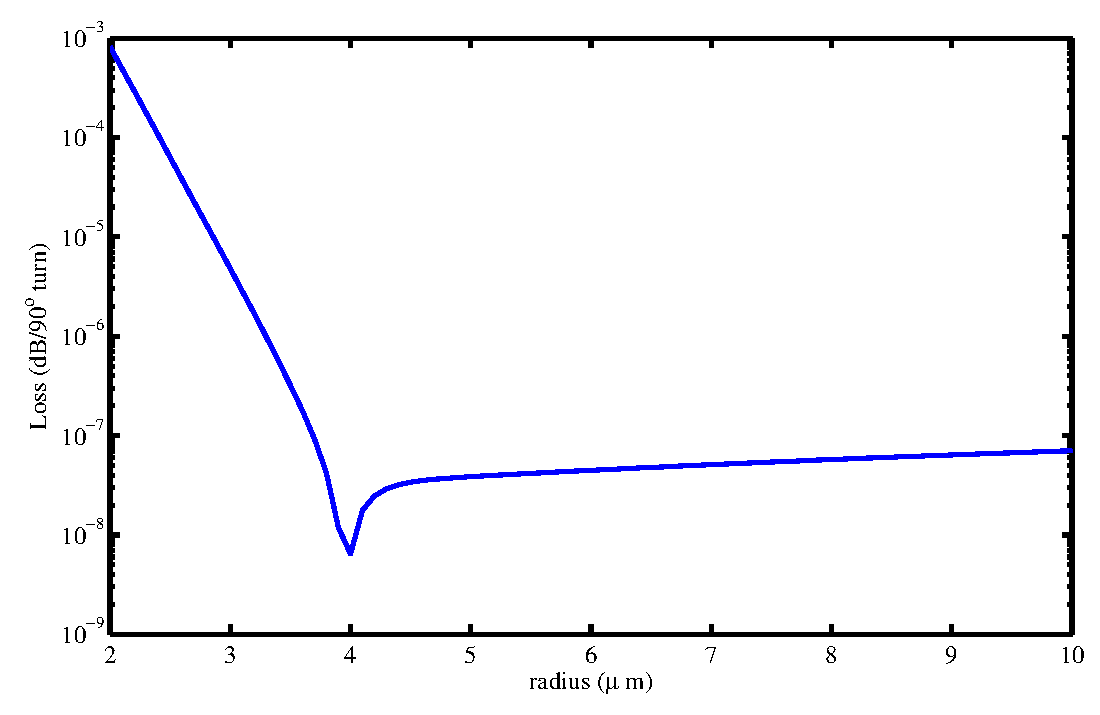
\includegraphics[width=12cm]{./Pictures/chapt5_deep_si_bend_loss.eps}
	\caption{在1550~nm处,不同弯曲半径下,转90$^\circ$导致的损耗(深刻蚀硅波导的尺寸450~nm宽,220~nm厚)}
	\label{chapt5_deep_si_bend_loss}
\end{figure}

我们在设计硅基可调反射镜与微环的波导尺寸参数与上一小结\ref{tunable_reflector}相同。除此之外,我们还需要考虑微环光调制器的整体尺寸。而影响微环整体尺寸的主要是需要考虑波导的弯曲半径。对于450~nm宽的条形硅波导,波导弯曲半径与转90$^\circ$引入的损耗,见图\ref{chapt5_deep_si_bend_loss}所示。可见半径为6~$\mu m$时,损耗已经可以忽略。因此,我们设计微环的整体长度为100~$\mu m$,使器件布局后满足6~$\mu m$的弯曲半径。

在反射相位调制区域,我们分析采用交趾(Interleaved)pn掺杂方式实现相位调制。根据Imec的工艺参数\cite{Imec},交趾pn掺杂的方式\cite{li2009silicon,pantouvaki2013comparison},在1550~nm处$V_\pi L = 0.8~V/cm$,也就意味着每伏电压使等效折射率有$1 \times  10^{-4}$的变化量。由于我们采用的集总电极的结构,这会使相位调制区形成驻波,电压加倍。因此,在集总电极的情况下,只需要0.5~V就能达到等效折射率$1 \times  10^{-4}$的变化量。如果采用差分驱动,驱动电压可以进一步降低\cite{Ding2013electro,zortman2011low}。

\begin{figure}[htb]
	\small
	\subfigure[微环内部有反射和无反射的透射谱]{
		\begin{minipage}[]{0.5\textwidth}
			\centering
			\label{chapt5_reflactor_modulator_k1}
			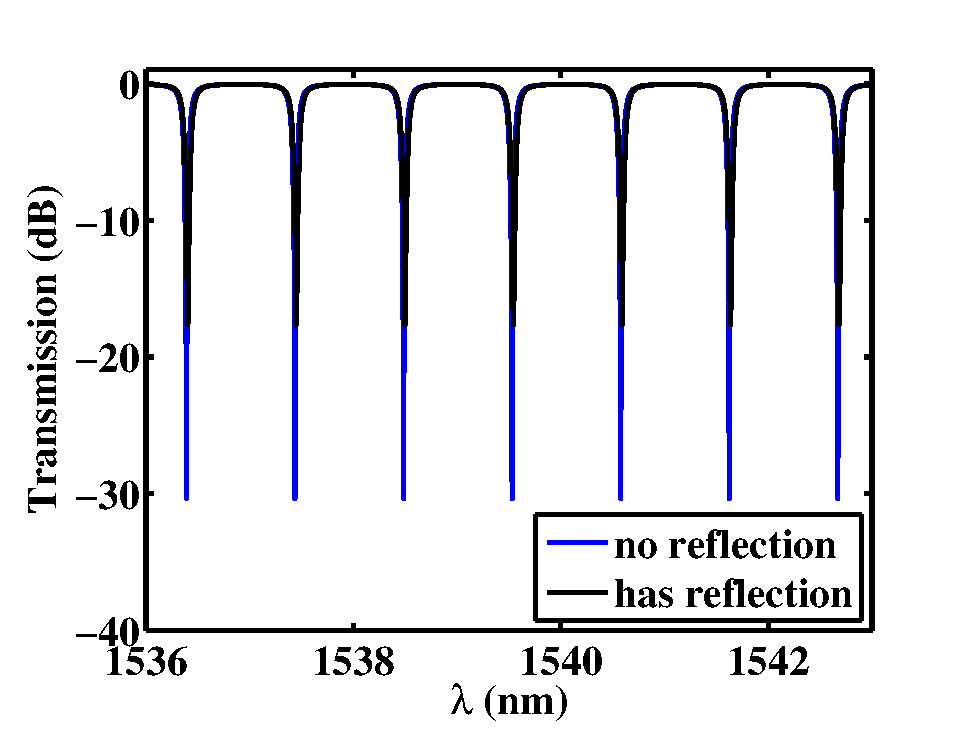
\includegraphics[width=8cm]{./Pictures/chapt5_reflactor_modulator_k1.eps}
		\end{minipage}}
	\subfigure[谐振波长$\lambda_c$附近透射谱的放大图]{
		\begin{minipage}[]{0.5\textwidth}
			\centering
			\label{chapt5_reflactor_modulator_k1_large} %% label for second subfigure
			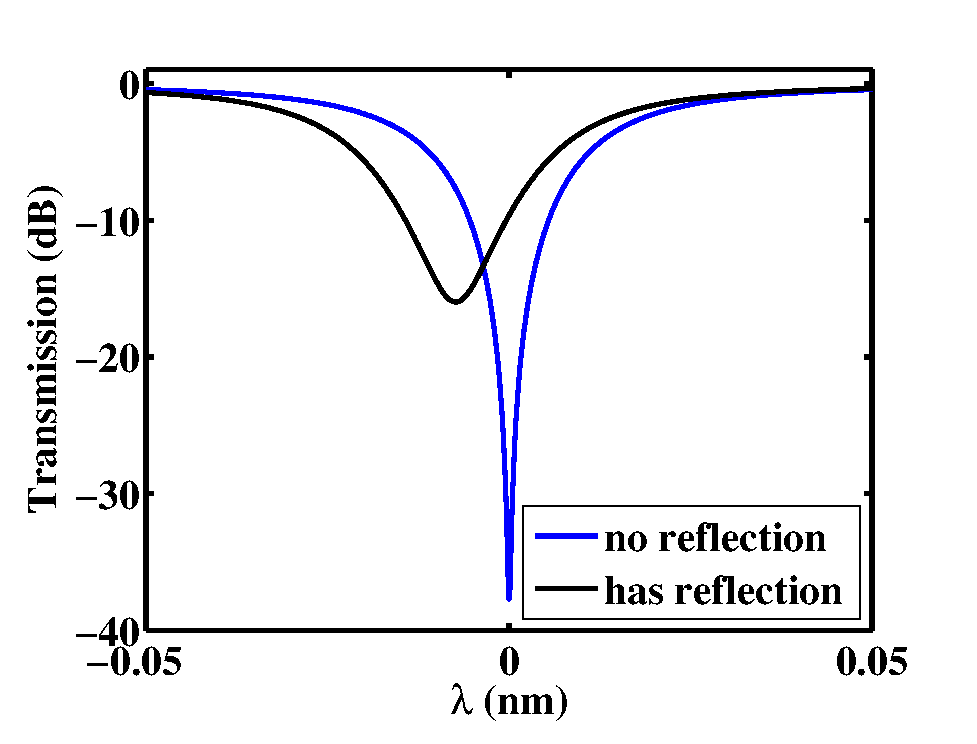
\includegraphics[width=8cm]{./Pictures/chapt5_reflactor_modulator_k1_large.eps}
		\end{minipage}}
	\subfigure[谐振波长$\lambda_c$附近调制的消光比]{
		\begin{minipage}[]{0.5\textwidth}
			\centering
			\label{chapt5_reflactor_modulator_k1_ER} %% label for second subfigure
			\includegraphics[width=8cm]{./Pictures/chapt5_reflactor_modulator_k1_ER.eps}
		\end{minipage}}		
	\subfigure[谐振波长$\lambda_c$附近调制的插入损耗]{
		\begin{minipage}[]{0.5\textwidth}
			\centering
			\label{chapt5_reflactor_modulator_k1_IL} %% label for second subfigure
			\includegraphics[width=8cm]{./Pictures/chapt5_reflactor_modulator_k1_IL.eps}
		\end{minipage}}			
	\caption{硅基可调反射镜的微环光调制器的在第一耦合系数$k_{i1}^2$ = 0.2的透射谱,调制消光比(Extinction Ratio, ER)和插入损耗(Insertion Loss,IL)}
	\label{chapt5_reflactor_modulator_k1_modulator}	
\end{figure}

\begin{figure}[htb]
	\small
	\subfigure[微环内部有反射和无反射的透射谱]{
		\begin{minipage}[]{0.5\textwidth}
			\centering
			\label{chapt5_reflactor_modulator_k2}
			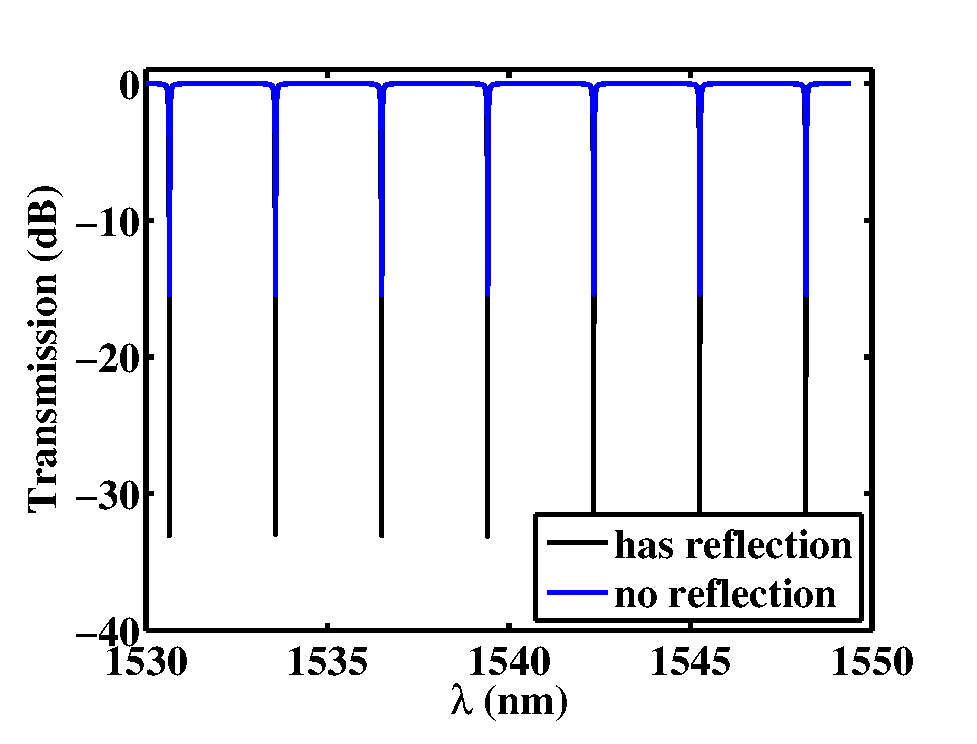
\includegraphics[width=8cm]{./Pictures/chapt5_reflactor_modulator_k2.eps}
		\end{minipage}}
	\subfigure[谐振波长$\lambda_c$附近透射谱的放大图]{
		\begin{minipage}[]{0.5\textwidth}
			\centering
			\label{chapt5_reflactor_modulator_k2_large} %% label for second subfigure
			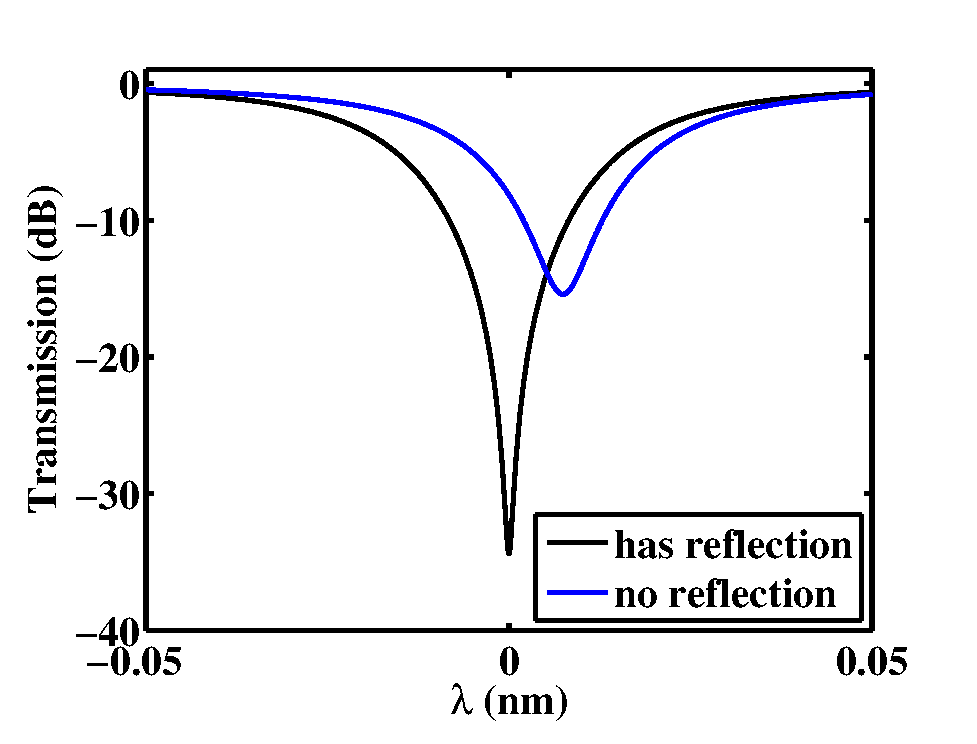
\includegraphics[width=8cm]{./Pictures/chapt5_reflactor_modulator_k2_large.eps}
		\end{minipage}}
	\subfigure[谐振波长$\lambda_c$附近调制的消光比]{
		\begin{minipage}[]{0.5\textwidth}
			\centering
			\label{chapt5_reflactor_modulator_k2_ER} %% label for second subfigure
			\includegraphics[width=8cm]{./Pictures/chapt5_reflactor_modulator_k2_ER.eps}
		\end{minipage}}		
	\subfigure[谐振波长$\lambda_c$附近调制的插入损耗]{
		\begin{minipage}[]{0.5\textwidth}
			\centering
			\label{chapt5_reflactor_modulator_k2_IL} %% label for second subfigure
			\includegraphics[width=8cm]{./Pictures/chapt5_reflactor_modulator_k2_IL.eps}
		\end{minipage}}			
	\caption{硅基可调反射镜的微环光调制器在第二耦合系数$k_{i2}^2$ = 0.26的透射谱,调制消光比(Extinction Ratio, ER)和插入损耗(Insertion Loss,IL)}
	\label{chapt5_reflactor_modulator_k2_modulator}	
\end{figure}	
我们继续采用Intercoonnect商业软件对整个器件的性能进行仿真计算。其中微环波导的耦合系数,可以选择两个值。耦合系数$k_{i1}$对应着微环内部没有反射时,谐振峰的透过率最低。此时,谐振峰低损耗状态是需要在相位调制器加电压,引入反射。耦合系数$k_{i2}$对应着微环内部有反射则谐振峰的透过率最低。而没有反射时,谐振峰处于透过状态。

图\ref{chapt5_reflactor_modulator_k1_modulator}展示了,当耦合系数处于第一个状态下($k_{i1}^2 = 0.2$),等效折射率差($\Delta n_{eff} = n_{eff1}-n_{eff2}$)从0变化到$1 \times  10^{-4}$,对应的反射率$r^2$从0 变化到了 0.0064时,透射谱的变化。从图\ref{chapt5_reflactor_modulator_k1}和局部放大图\ref{chapt5_reflactor_modulator_k1_large}可以看到,由于可调反射器反射谱宽的特性,所有谐振波长都会受到显著的强度调制。该调制器谐振峰之间的间距为1 nm,如果我们在微环上加入热电极,就可以调节谐振波长的位置,从而实现宽光学带宽的调制。图\ref{chapt5_reflactor_modulator_k1_ER}展示了在谐振波长附近的调制消光比(为图\ref{chapt5_reflactor_modulator_k1_large}中两条曲线的差值。)。可以看到对于谐振波长$\lambda_c$,调制器消光比达到了19~dB,而此时的插入损耗为10~dB。这个插入损耗可以通过改进工艺,降低波导的损耗,从而使微环的谐振峰,在有内部反射的情况下,损耗降低。另外,由于谐振峰处的光子寿命长,会影响调制速度,因此实际应用中,工作波长也会偏离谐振峰处。

我们同样分析了,当微环处于第二个可选耦合系数($k_{i2}^2 = 0.26$)下,器件的透射谱,消光比和插入损耗,见图\ref{chapt5_reflactor_modulator_k2_modulator}所示。从图\ref{chapt5_reflactor_modulator_k2}和图\ref{chapt5_reflactor_modulator_k2_large}可以看出,在这个耦合系数下,调制其的透射谱几乎和图\ref{chapt5_reflactor_modulator_k1}和图\ref{chapt5_reflactor_modulator_k1_large}的保持一致,除了两个工作状态下的谐振峰的消光比互换。

\begin{figure}[htb]
	\centering
	\includegraphics[width=12cm]{./Pictures/chapt5_tunable_reflection_ring_modulator_equit_circuit.jpg}
	\caption{基于集总电极的硅基可调反射镜的微光环调制器等效电路模型}
	\label{chapt5_tunable_reflection_ring_modulator_equit_circuit}
\end{figure}
\begin{figure}[htb]
	\centering
	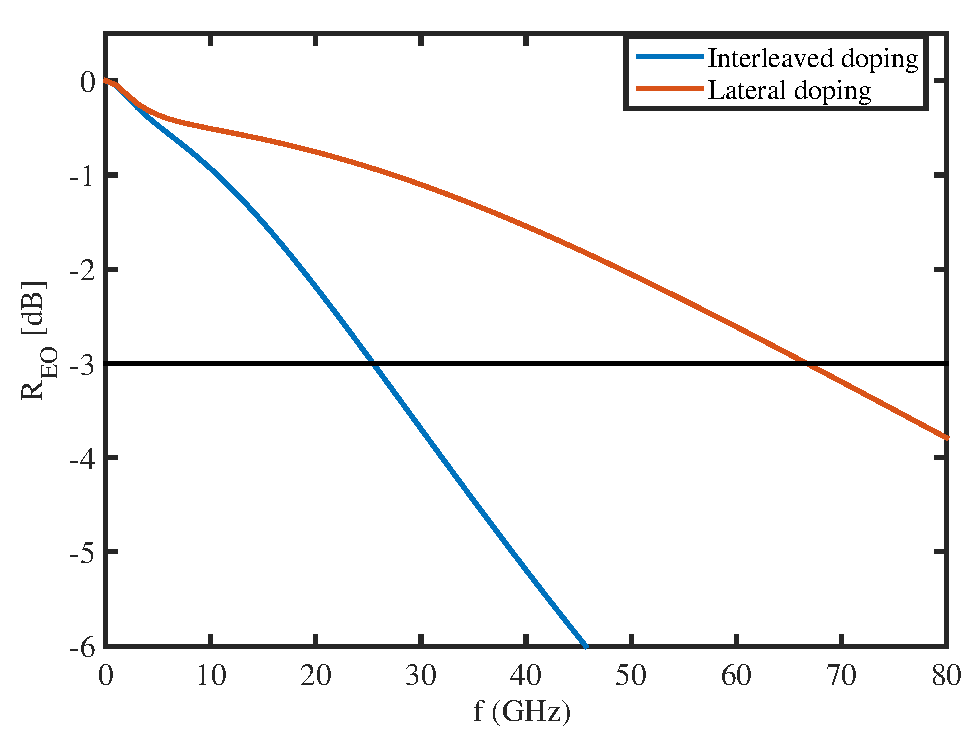
\includegraphics[width=12cm]{./Pictures/chapt5_bandwidth.eps}
	\caption{利用200~$\mu m$长的集总电极的硅基可调反射镜的微环光调制器,在交趾pn掺杂下,电光调制的频谱响应($R_{EO}$)}
	\label{chapt5_bandwidth}
\end{figure}

虽然这个新型光调制器工作原理和微环光调制器不一样,但是也具有光学谐振腔。因此,我们将分别从电学RC限制的调制带宽和谐振腔光子寿命限制的调制带宽分析。我们将先分析调制器电学RC限制的3~dB调制带宽。光调制器的电路模型如图\ref{chapt5_tunable_reflection_ring_modulator_equit_circuit}所示。其中,$C_p$为用于接触探针的电极焊盘(pad)的寄生电容,$R_s$,$C_s$为金属电极的寄生电阻,电容。$L_j$,$R_j$和$C_j$分别为pn结的寄生电感,串联电阻和结区电容。该光调制的电光响应$R_{EO}$公式\ref{Equ:R_EO_ring}所示。
\begin{equation}
\label{Equ:R_EO_ring}
R_{EO} = \left|\frac{R_{tot}}{R_{tot}+Z_s}\cdot\frac{1}{1-\omega^2C_jL_j+j\omega C_j R_j}\right|^2
\end{equation}
其中,$R_{tot}$为等效电路中器件的总电阻;$Z_s$为射频源的输出阻抗,50 $\Omega$;对于交趾掺杂的相位调制器,依据Imec公司\cite{Imec}提供的电阻、电容的参数为:$C_p = 9.3~fF$, $C_s = 56.4~fF$, $Rs = 904~\Omega$, $L_j = 0.0142~nH$, $R_j = 8.85~\Omega\cdot mm$, $C_j = 563.6~fF/mm$。因此,我们计算得到的有电学RC限制的电光调制带宽($R_{EO}$)如图\ref{chapt5_bandwidth}所示,对应的3~dB带宽为14~GHz。

然后,我们分析谐振腔光子寿命限制对调制带宽的影响。我们采用时域耦合耦合理论,先根据文献[\citenum{pile2014small}]的思路推导了微环中存在反射时,光子寿命对带宽的影响。当调制器被正弦信号驱动时,输出的光信号将有两个旁瓣$S_{t}^+$和$S_{t}^-$,其频率分别为$\omega_0+\omega_m$和$\omega_0-\omega_m$。$\omega_0$为输入光的角频率,$\omega_m$为调制信号的角频率。输出光可以写成公式\ref{Equ:St_m}的形式。
\begin{equation}
\label{Equ:St_m}
S_t = S_{t0}e^{j\omega_0t}+S_{t1}^+\frac{e^{j(\omega_0+\omega_m)t}}{2}+S_{t1}^-\frac{e^{j(\omega_0-\omega_m)t}}{2}
\end{equation}

我们接着就可以获得调制后输出光功率的表达式:
\begin{equation}
\label{Equ:Pout_m}
P_{out} = |S_{t0}|^2+Re\left[(S_{t0}^*S_{t1}^{+}+S_{t0}S_{t1}^{-*})e^{j\omega_mt} \right]=|S_{t0}|^2+Re\left[H(\omega_m)\Delta n e^{j\omega_mt}\right]
\end{equation}
其中,第一项$|S_{t0}|^2$为直流信号,而$|H(\omega_m)|^2$为器件的调制响应函数,具体表达式如公式\ref{Equ:Homega_m}所示。
\begin{equation}
\label{Equ:Homega_m}
 |H(\omega_m)|^2 = |(S_{t0}^*S_{t1}^{+}+S_{t0}S_{t1}^{-*})/\Delta n|^2 
\end{equation}

因此,我们只需要获得$S_{t0}$,$S_{t1}^+$,和$S_{t1}^-$就可以计算得到调制响应函数。第一步,我们将公式\ref{Equ:St_m}代入公式\ref{Equ:alpha_ccw}和公式\ref{Equ:alpha_cw}就可以获得调制器处于动态工作下的tCMT方程。我们忽略高次谐波项,再根据谐振频率进行分类,可以获得6组方程。6组方程我们将其分为3对,第一对方程组为正向和反向的直流信号,分别关于$\alpha_+$和$\alpha_-$的方程组。此方程组与公式\ref{Equ:alpha_ccw}和公式\ref{Equ:alpha_cw}相同。

第二对方程组为正向和反向振幅被调制产生的$\omega_0+\omega_m$上旁瓣信号,分别为$\alpha_+^+$和$\alpha_-^+$,对应的方程组\ref{eq:1}。
\begin{subequations}  \label{eq:1}
	\begin{align}  
	&j(\omega_0+\omega_m)\alpha_+^+ = (j\omega_r-1/\tau)\alpha_+^+ +j\Delta \omega_r\alpha_+ - j\Delta \mu_r\alpha_- - j\mu_r\alpha_-^+            \label{eq:1A} \\
	&j(\omega_0+\omega_m)\alpha_-^+ = (j\omega_r-1/\tau)\alpha_-^+ +j\Delta \omega_r\alpha_- - j\Delta \mu_r^*\alpha_+ - j\mu_r^*\alpha_+^+           \label{eq:1B}
	\end{align}
\end{subequations}

第三对方程组为正向和反向振幅被调制产生的$\omega_0-\omega_m$下旁瓣信号,分别为$\alpha_+^-$和$\alpha_-^-$,对应的方程组\ref{eq:2}。
\begin{subequations}  \label{eq:2}
	\begin{align}  
	&j(\omega_0-\omega_m)\alpha_+^+ = (j\omega_r-1/\tau)\alpha_+^- +j\Delta \omega_r\alpha_+ - j\Delta \mu_r\alpha_- - j\mu_r\alpha_-^-            \label{eq:2A} \\
	&j(\omega_0-\omega_m)\alpha_-^- = (j\omega_r-1/\tau)\alpha_-^- +j\Delta \omega_r\alpha_- - j\Delta \mu_r^*\alpha_+ - j\mu_r^*\alpha_+^-           \label{eq:2B}
	\end{align}
\end{subequations}

分别求解这三对方程组我们可以获得$\alpha_+$,$\alpha_-$,$\alpha_+^+$和$\alpha_+^-$,如下所示:
\begin{subequations}  \label{eq:3}
	\begin{align}  
	&\alpha_+ = -j\mu_iS_i \frac{j\delta+\frac{1}{\tau}}{(j\delta+\frac{1}{\tau})^2+|\mu_r|^2}  	\label{eq:3A}\\
	&\alpha_- = -\mu_i\mu_r^*S_i \frac{1}{(j\delta+\frac{1}{\tau})^2+|\mu_r|^2}  	\label{eq:3B}\\	
	&\alpha_+^+ = \frac{j(\delta+\omega_m)+\frac{1}{\tau}}{((j\delta+\omega_m)\frac{1}{\tau})^2+|\mu_r|^2}\left[\mu_r\frac{\Delta \omega_r\alpha_- - \Delta\mu_r^*\alpha_+}{j(\delta+\omega_m)+\frac{1}{\tau}} + j\Delta \omega_r \alpha_+ -j\Delta\mu_r\alpha_-\right]             \label{eq:3C}\\
	&\alpha_+^- = \frac{j(\delta-\omega_m)+\frac{1}{\tau}}{((j\delta-\omega_m)\frac{1}{\tau})^2+|\mu_r|^2}\left[\mu_r\frac{\Delta \omega_r\alpha_- - \Delta\mu_r^*\alpha_+}{j(\delta-\omega_m)+\frac{1}{\tau}} + j\Delta \omega_r \alpha_+ -j\Delta\mu_r\alpha_-\right]             \label{eq:3D}	
	\end{align}
\end{subequations}
其中,$\delta = \omega_0-\omega_r$为工作频率和谐振频谱的差距;$\Delta \omega_r = -\Delta n \omega_r /n_g$为调制折射率导致的谐振腔谐振频率的漂移量;$\Delta \mu_r = \omega_0 L_m \Delta n/(n_g L_{tot})$为调制折射率导致的反射耦合强度的变化量。$L_m = 200~\mu m$为调制区域的长度,$L_{tot} = 550~\mu m$为整体器件的长度。接着我们将公式\ref{eq:3}带入到公式\ref{eq:4},就可以获得$S_{t0}$,$S_{t1}^+$,和$S_{t1}^-$,从而根据公式\ref{Equ:Homega_m}计算得到硅基反射微环光调制器的频率响应函数$|H(\omega_m)|^2$。
\begin{subequations}  \label{eq:4}
	\begin{align}  
	&S_{t0} = S_i-j\mu_i\alpha_+  	\label{eq:4A}\\
	&S_{t1}^+ = -j\mu_i\alpha_+^+ 	\label{eq:4B}\\	
	&S_{t1}^- = -j\mu_i\alpha_+^-            \label{eq:4C}	
	\end{align}
\end{subequations}

\begin{figure}[htb]
	\small
	\subfigure[]{
	\begin{minipage}[]{0.5\textwidth}
		\centering
		\label{chapt5_optical_eo_band}
		\includegraphics[width=8cm]{./Pictures/chapt5_optical_eo_band.eps}
	\end{minipage}}
	\subfigure[]{
	\begin{minipage}[]{0.5\textwidth}
		\centering
		\label{chapt5_optical_total_band} %% label for second subfigure
		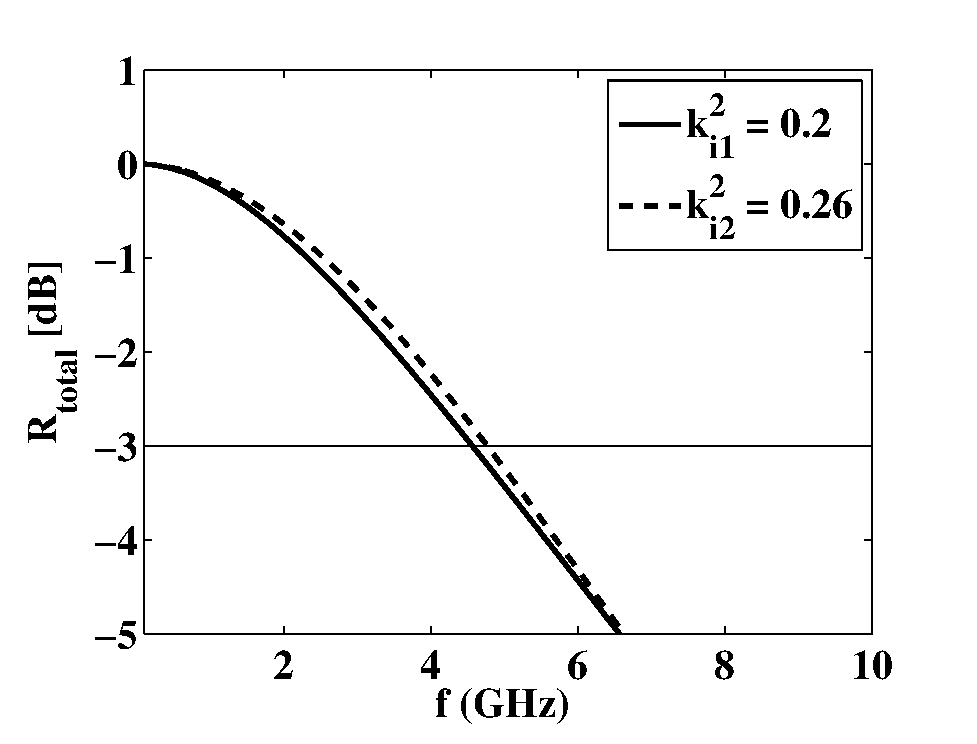
\includegraphics[width=8cm]{./Pictures/chapt5_optical_total_band.eps}
	\end{minipage}}
	\caption{当工作波长和谐振峰的偏移量为10 pm时,两种耦合系数下器件的调制频率响应。(a)光子寿命限制的频率响应;(b)器件电学和光学整体的频率响应}
	\label{chapt5_optical_oe_total_band}	
\end{figure}
				
由于谐振峰处的光子寿命最长,所以对应的调制带宽最小。因此,在综合考虑插入损耗,消光比下,我们选取的工作波长和谐振峰的偏移量为10 pm。从图\ref{chapt5_reflactor_modulator_k1_modulator}可以看出,耦合系数为$k_{i1} = 0.2$时,消光比和插入损耗分别为 5 dB 和 6 dB。从图\ref{chapt5_reflactor_modulator_k2_modulator}可以看出,耦合系数为$k_{i2} = 0.26$时,消光比和插入损耗分别为 8 dB 和 6 dB。两个耦合系数下由光子寿命限制的频率响应$|H(\omega_m)|^2$见图\ref{chapt5_optical_eo_band}所示。可以看到光子寿命对调制带宽影响大于电学RC常数对调制带宽的影响,两个耦合系数的3 dB调制带宽都在5.7 GHz左右。 耦合系数大的3 dB带宽偏大的。其原因是耦合增大,对应的耦合损耗增加,从而使光子寿命减小,调制带宽增大。我们将电学RC限制的频率响应和光子寿命限制的频率响应相乘,就可以获得器件整体的频率响应$R_{total} = |H(\omega_m)|^2 R_{EO}$,如图\ref{chapt5_optical_total_band}所示。从中可以看到两个耦合系数下的3 dB调制带宽都减小到 4.8 GHz左右。

通过比较插入损耗,消光比和带宽,我们可以发现这种光调制器工作在耦合系数为$k_{i2}$下的综合性能略优于工作在耦合系数$k_{i1}$下的综合性能。它具有在0.5V 驱动电压下, 8 dB的消光比,6 dB的插入损耗, 4.8 GHz的3 dB调制带宽。

\section{本章小结}
在本章中,我们首先通过时域耦合模理论,宏观上分析了微环中反射对透射谱的影响。可以看到对于高Q值,并且工作在临界耦合点的微环,内部微小的反射,对谐振波长的透射率有显著提高。然后我们在微环中引入光栅结构,实验上分析了微环中的不同反射强度对微环的透射率以及谐振峰劈裂的影响。我们利用频域的传输矩阵也计算了含光栅微环的透射谱,计算结果与实验结果相吻合。接着,我们设计并分析了硅基可调反射镜的结构,实现了宽光谱范围的可调反射。并且分析了这种可调反射镜结构的工艺容差。最后,我们将可调反射镜与微环相结合,分析了不同波导与微环耦合系数对调制器的静态消光比,插入损耗和动态电光调制带宽的影响。通过分析,我们计算了在交趾pn掺杂模式下,调制器在0.5 V驱动电压下能实现8 dB的消光比。并且我们还首次分析了在调制微环内部反射率下,光子寿命对带宽的影响。最后综合考虑电学带宽和光子寿命带宽,我们发现目前的硅基反射微环光调制器的3 dB带宽受到光子寿命的限制为4.8 GHz。

